\documentclass[11pt]{article}
\usepackage[margin=1in]{geometry}
\usepackage[T1]{fontenc}
\usepackage{lmodern}
\usepackage{graphicx}
\usepackage{booktabs}
\usepackage{xcolor}
\usepackage{tcolorbox}
\usepackage{caption}
\usepackage{enumitem}
\usepackage[numbers,sort&compress]{natbib}
\usepackage[hidelinks]{hyperref}
\usepackage{titlesec}
\usepackage{float}

\graphicspath{{../results/figs/}}
\definecolor{accent}{HTML}{B43C7A}
\definecolor{ink}{HTML}{26251F}
\definecolor{muted}{HTML}{6F6F69}
\definecolor{card}{HTML}{E6E3DC}
\titleformat{\section}{\large\bfseries\color{accent}}{\thesection}{0.6em}{}
\titleformat{\subsection}{\normalsize\bfseries}{\thesubsection}{0.6em}{}
\captionsetup{font=small,labelfont=bf,width=0.95\textwidth}
\setlist{nosep,leftmargin=*}
\setlength{\parskip}{4pt}

\newcommand{\todo}[1]{\textcolor{accent}{[TODO: #1]}}

\title{\vspace{-1.2em}Do confident-but-wrong answers leave an internal signature?\\
\large Literature review, hypotheses, and experiment design\\[-2pt]
\normalsize EE 456 honors option, checkpoint 1 (October 16, 2026)}
\author{Ameya Panchal\quad\textcolor{muted}{advisor: Dr.\ David J.\ Miller}}
\date{}

\begin{document}
\maketitle
\vspace{-2.5em}

\begin{tcolorbox}[colback=card,colframe=card,arc=2pt,left=8pt,right=8pt,top=6pt,bottom=6pt]
\textbf{Question.} When an LLM answers wrongly \emph{and} confidently, does its activation space carry a signal that output-side hallucination monitors cannot reach?

\textbf{Hypothesis.} A linear readout of the residual stream separates confident-correct from confident-wrong answers better than any score derived from the output distribution (H1); and the direction that encodes ``wrong'' is distinct from the direction that encodes ``confident'' (H2), in the sense of CSO-LLM's cosine criterion.

\textbf{Status.} Pilot on Qwen3-0.6B and Qwen3-4B, 2{,}000 closed-book TriviaQA questions. H1 is supported: on the answers where probability is high and five samples agree, a linear probe scores 0.76 AUROC and every output-side score sits at 0.50--0.59. H2 splits by model: distinct directions at 0.6B, largely shared at 4B. Labels are lexical and not yet audited.

\textbf{Everything here is reproducible} from \texttt{notebooks/lit\_review.ipynb} in the project repository; figure numbers in that notebook are given in each caption.
\end{tcolorbox}

\section{The question and the hypotheses}

Dr.\ Miller's CSO-LLM work found that, in a sentiment classifier, decoy words move a model's activations \emph{along} the negative-to-positive axis while backdoor triggers move them \emph{off} it; a cosine penalty on that displacement separates the two. The question of this project is whether hallucination has the same shape. We define a hallucination narrowly as a \textbf{confident, incorrect} answer, which is the case that matters in practice and the case where current monitors are weakest. Three hypotheses are pre-registered.

\begin{itemize}
  \item \textbf{H1 (internal signal exists).} On the subset of answers the model gives with first-token probability $\ge 0.8$, a linear probe on the residual stream reaches an AUROC whose 95\% bootstrap lower bound exceeds both 0.55 and the token-probability baseline on that subset.
  \item \textbf{H2 (it is directional).} The mean-difference axis for correctness (correct $-$ wrong, estimated within confident answers) is not parallel to the axis for confidence (confident $-$ uncertain, estimated within correct answers): its cosine falls at or below a shuffled-label null.
  \item \textbf{H0 (informative null).} If H1 fails, confident errors are not linearly separable from confident successes in the residual stream, and the final report characterizes where existing monitors fail instead.
\end{itemize}

\section{What the literature says}

Three papers carry the argument; they are read in the order the argument runs: hallucination as uncertainty, the blind spot of uncertainty, and the internal signal. Each subsection states the paper's claim, shows the same measurement on our own pilot, and says what it gives us.

\subsection{Hallucination as uncertainty: semantic entropy \citep{farquhar2024semantic}}

\textbf{Claim.} Sample several answers, cluster them by meaning, and take the entropy over clusters. High semantic entropy (SE) means the model does not have one answer, and such answers are usually wrong. SE beats naive token entropy and the model's own self-assessment (p(True) \citep{kadavath2022know}) at predicting wrong answers on TriviaQA and other short-form QA. The authors scope the method to \emph{confabulations}, errors that vary between samples; they say explicitly that it is not designed for errors the model makes consistently.

\begin{figure}[H]\centering
  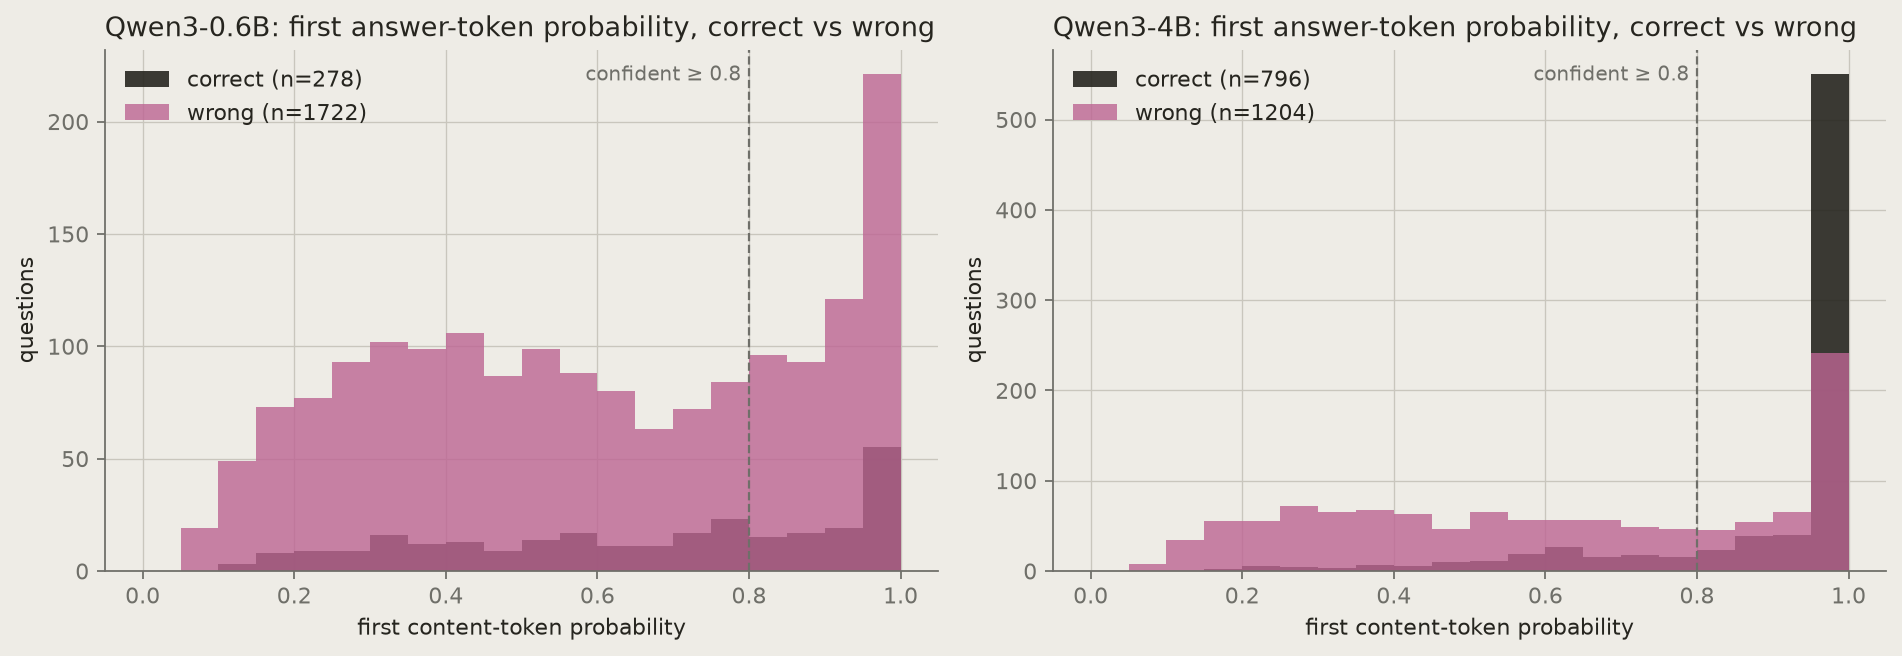
\includegraphics[width=0.9\textwidth]{01_confidence_hist}\\[4pt]
  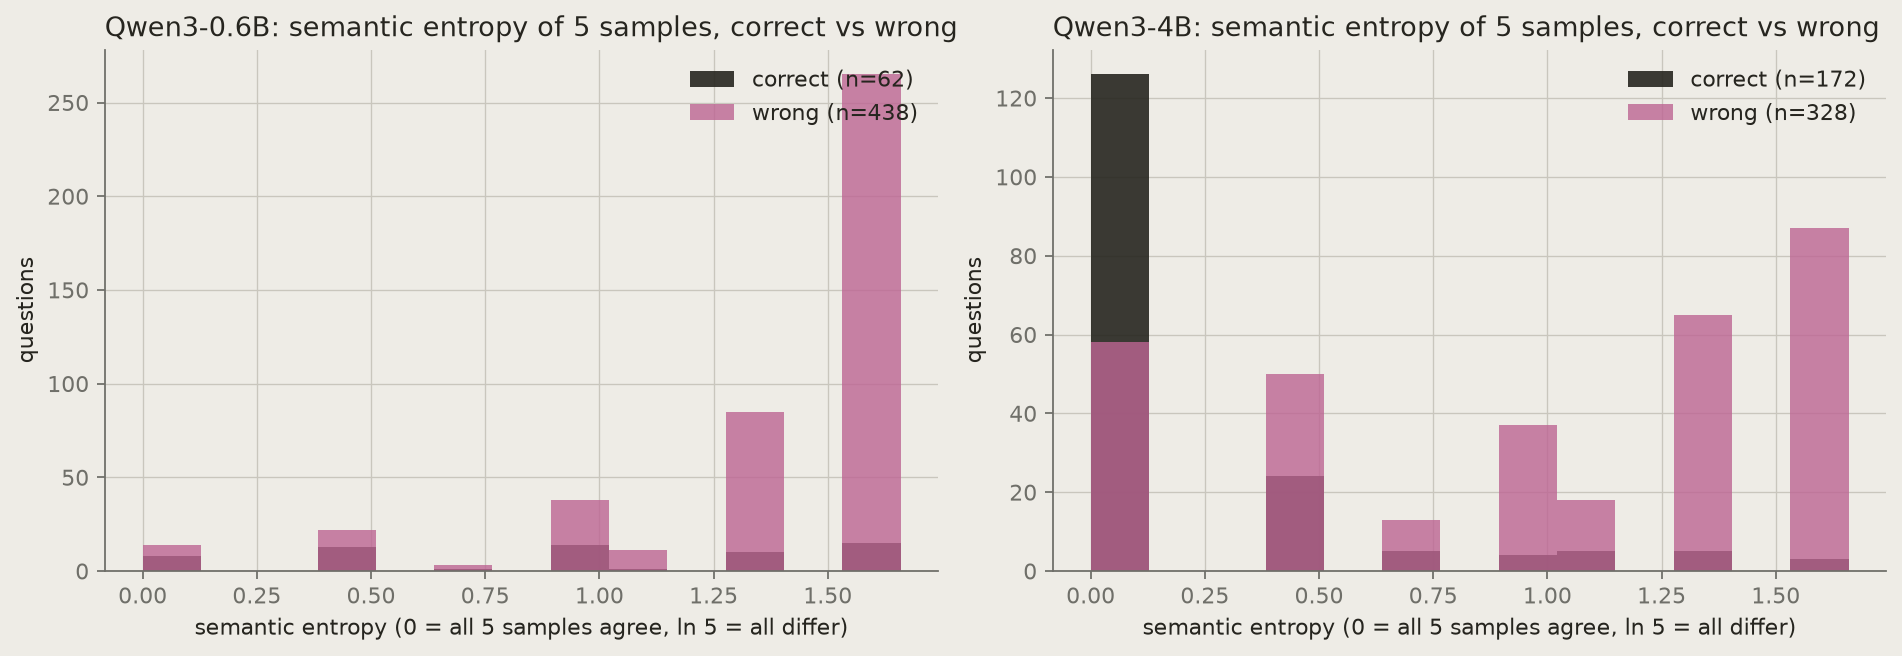
\includegraphics[width=0.9\textwidth]{05_semantic_entropy_hist}
  \caption{Top: first-answer-token probability for correct (dark) and wrong (pink) answers; the vertical line is the ``confident'' cut. Bottom: semantic entropy of five samples per question (500 questions). Wrong answers skew to high entropy, as the paper reports, but the zero-entropy bin contains both colours. Notebook Figures 1 and 5.}
\end{figure}

\textbf{What it gives us.} The cleanest statement of the uncertainty view and its own boundary. If a model repeats the same wrong answer every time, SE is zero by construction, so the method cannot see that error. That population is exactly our definition of hallucination.

\subsection{The blind spot: high-certainty hallucinations \citep{simhi2025choke}}

\textbf{Claim.} CHOKE (Certain Hallucinations Overriding Known Evidence) is the case where a model answers a question correctly under most phrasings, a trivial rephrasing flips it, and the wrong answer comes out with high certainty. Earlier work by the same group \citep{simhi2024ignorance} separates errors made \emph{despite} knowing the answer (HK$^{+}$) from errors of ignorance (HK$^{-}$) with exactly such paired prompts. Across Mistral-7B, Llama-3.1-8B and Gemma-2-9B, CHOKE is 16--43\% of HK$^{+}$ errors on Natural Questions and 8--26\% on TriviaQA (their Tables 1 and 4), and the examples are consistent across prompts. Most relevant for us: of the mitigation families they test, certainty-based and prompting methods drop sharply on CHOKE, while a linear probe on the residual stream is the one method that ``remains stable across all metrics'' (their Section 5.2, Figure 5b), and their own proposed fix is a probe trained with CHOKE examples oversampled.

\begin{figure}[H]\centering
  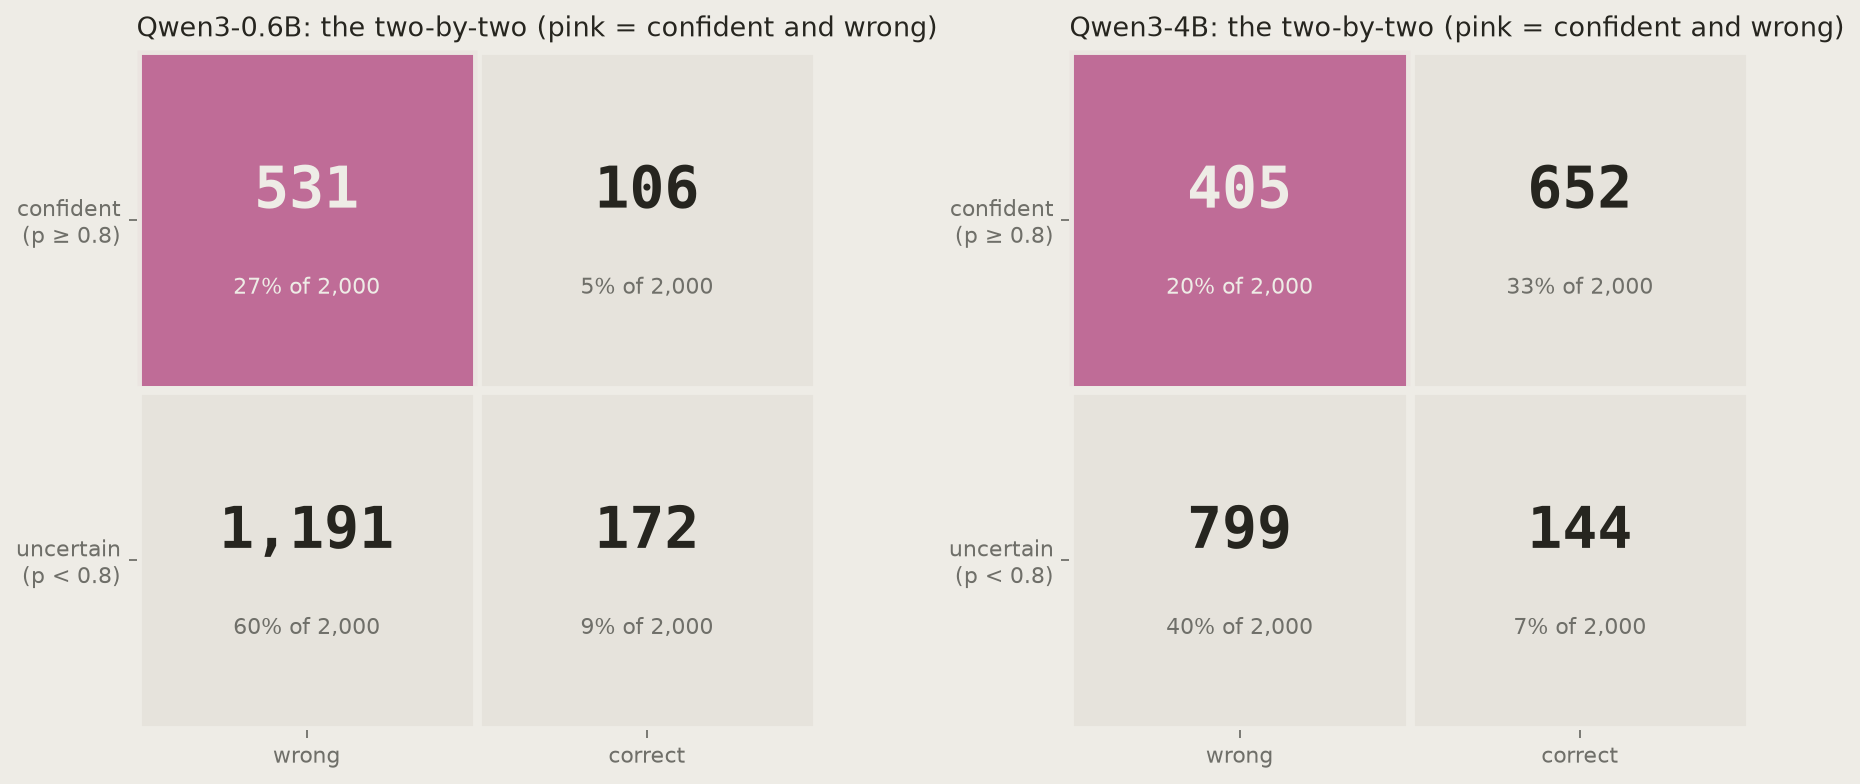
\includegraphics[width=0.9\textwidth]{10_quadrants}\\[4pt]
  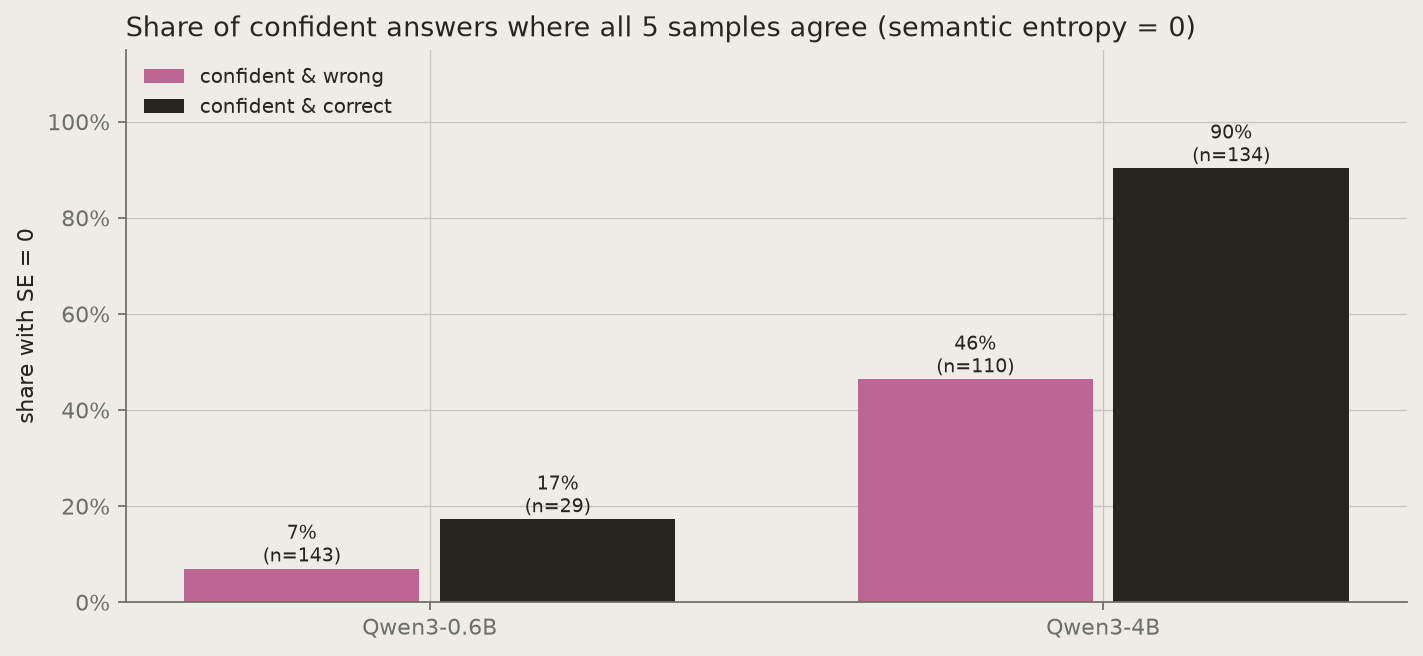
\includegraphics[width=0.75\textwidth]{09_se_zero_share}
  \caption{Top: the two-by-two on our pilot. The pink cell is confident-and-wrong: 531 of 2{,}000 at 0.6B, 405 at 4B. Bottom: at 4B, 90\% of confident-correct answers are stable under sampling but only 46\% of confident-wrong ones are; the pink bar is the share of confident errors that semantic entropy cannot see at all. Notebook Figures 10 and 9.}
\end{figure}

\textbf{What it gives us.} The population to study, the first evidence that probes are the right tool for it, and a warning. One distinction matters: CHOKE proper requires showing the model \emph{knew} the answer, which needs paired prompts. Our pilot population is the broader ``confident and wrong'' set, which also contains errors of ignorance; it is 20--27\% of all questions and does not shrink much when the confidence threshold is raised (Figure~\ref{fig:sweep}). Narrowing it to CHOKE proper is the November 6 experiment. The warning is that ``confident'' by output probability is not the same as ``certain'': at 0.6B almost no confident answer is stable under sampling, so output probability is a poor proxy for model certainty in small models.

\subsection{The internal signal: probes on hidden states \citep{orgad2025know}}

\textbf{Claim.} Linear probes on the hidden state at the \emph{exact answer token} predict correctness better than any output-based score, with the best layers in the middle-to-late stack. The model can internally encode the right answer while emitting the wrong one. Probes do not transfer across task types, so ``truthfulness'' is not one universal feature. Related work finds a single ``truth direction'' with difference-of-means \citep{marks2023geometry,burger2024truth}.

\begin{figure}[H]\centering
  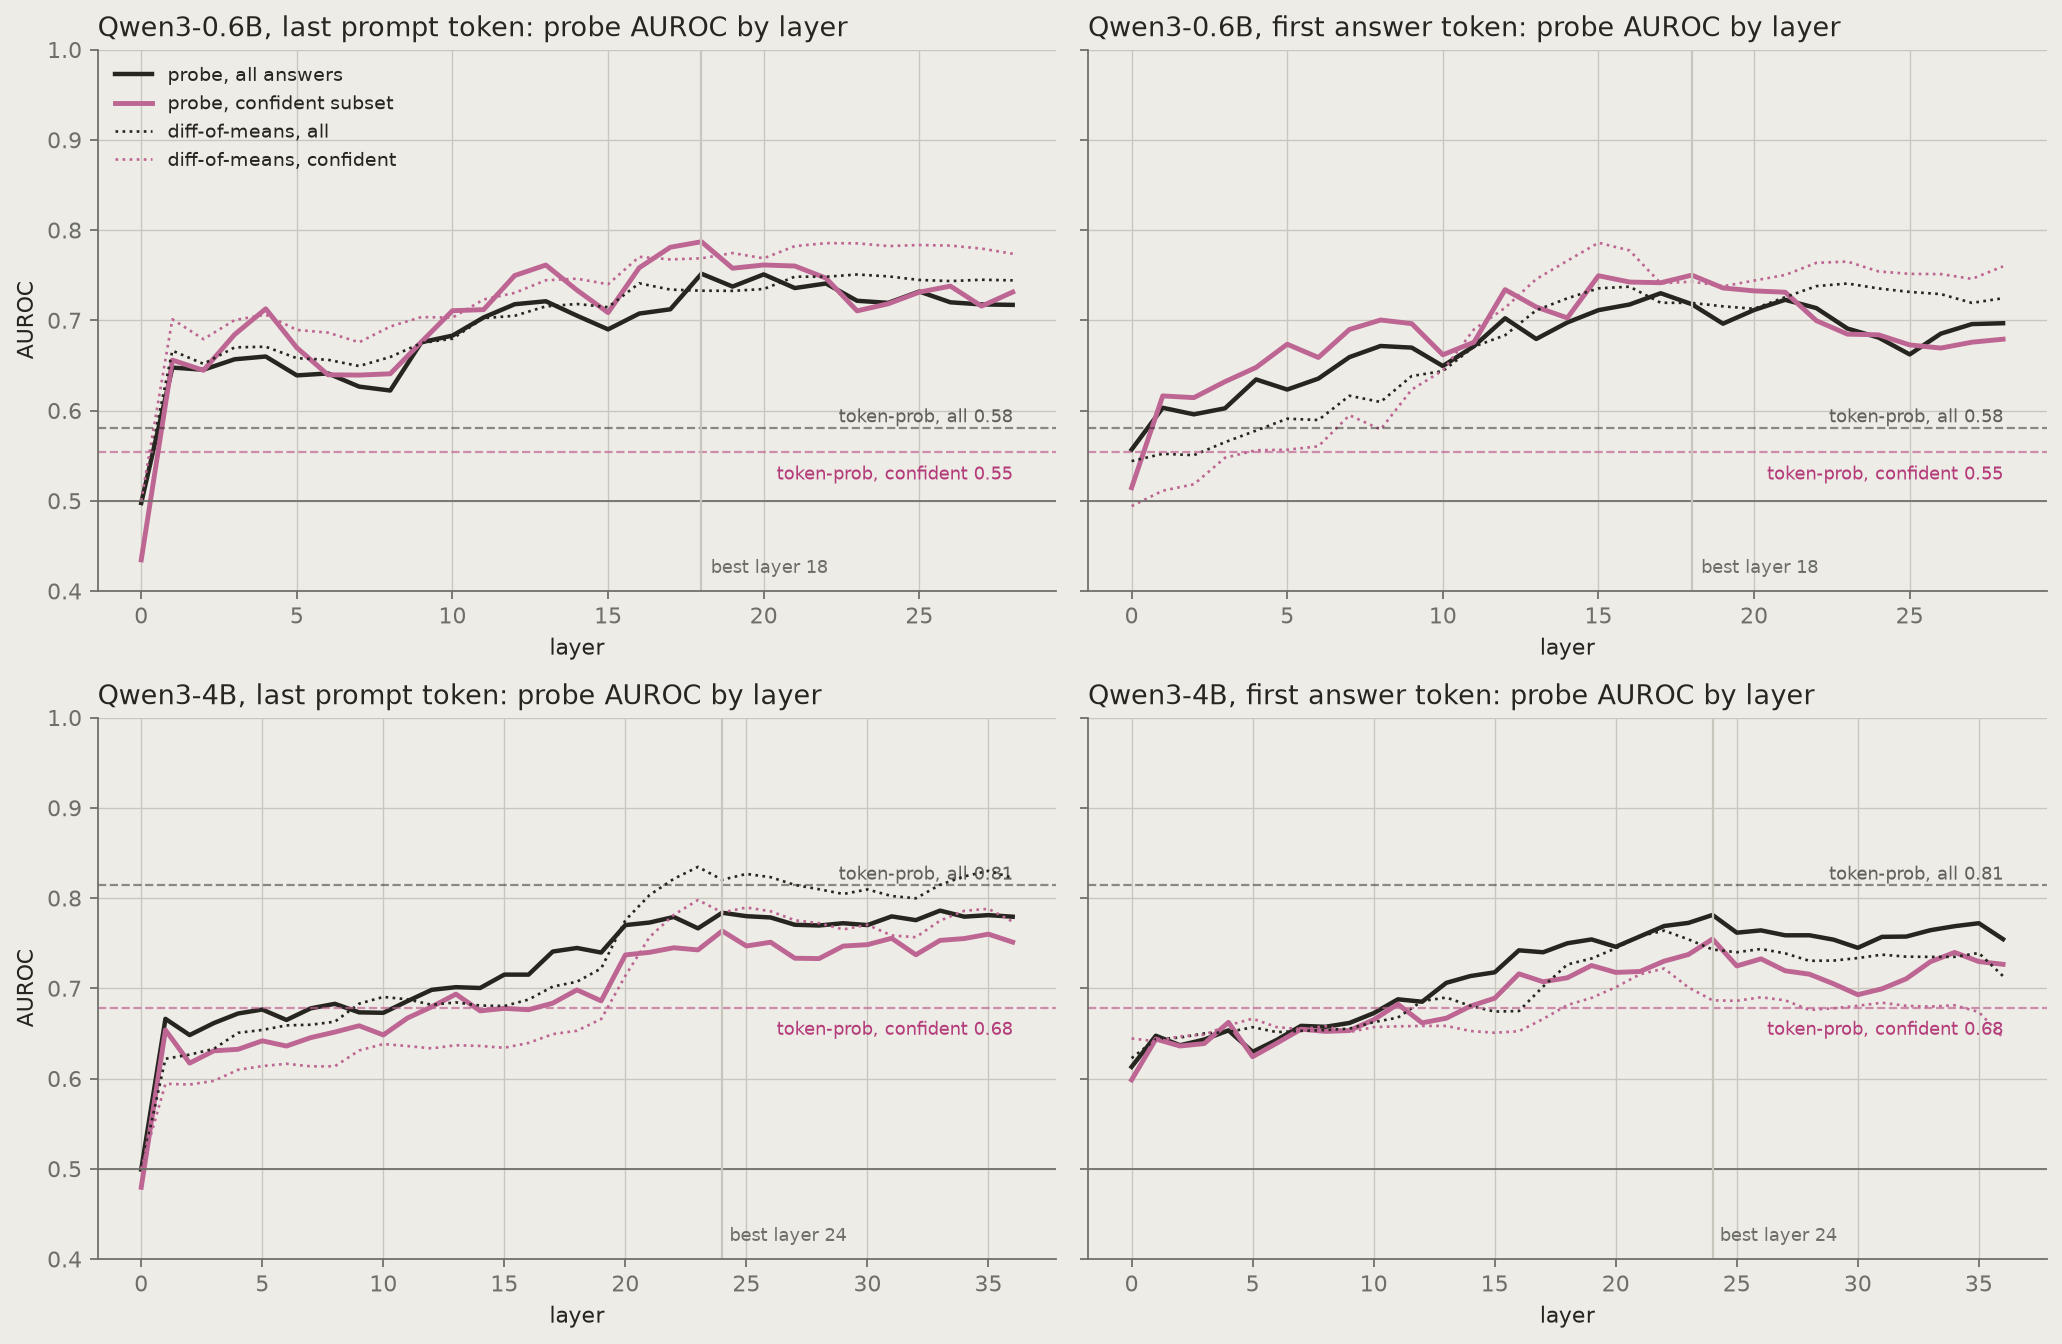
\includegraphics[width=0.98\textwidth]{14_probe_auroc_by_layer}
  \caption{Out-of-fold probe AUROC by layer on our pilot, two models and two token positions. Solid pink: probe on the confident subset. Dashed pink: token probability on the same subset. Best layers are 18 of 28 (0.6B) and 24 of 36 (4B), both at about two-thirds depth. Layer 18 is also the layer CSO-LLM selected for Qwen3-0.6B. Notebook Figure 14.}
\end{figure}

\textbf{What it gives us.} The method (a 5-fold out-of-fold logistic probe), the token position to read, the expectation that middle layers carry the signal, and a caveat we inherit: \citet{janiak2025illusion} show that lexical correctness labels inflate detector scores, with drops of up to 46\% when an LLM judge replaces lexical overlap, so an LLM-judge audit is required before any number here is final.

\subsection{Where CSO-LLM enters, and the gap}

CSO-LLM \citep{li2026cso} penalises candidate trigger tokens whose activation perturbation points \emph{along} the direction of the putative target class; its criterion is a \emph{per-pair} displacement cosine: for a prompt and its perturbed twin, the cosine between the activation displacement and a reference axis. Nothing in the hallucination-monitor literature we reviewed applies a directional criterion of this kind. Probes ask ``is there a separating hyperplane''; CSO asks ``which way did the point move, relative to the axis that normal variation uses.'' The gap is therefore concrete: \textbf{no one has asked whether confident errors displace activations off the confidence axis.} Answering it needs paired prompts (the CHOKE protocol), which is the November 6 experiment. The population-level version, comparing the correctness axis to the confidence axis, can be done now and is reported in Section~\ref{sec:directions}.

\subsection{The four questions the honors form asks of this phase}

\begin{table}[H]\centering\small
\begin{tabular}{p{0.30\textwidth}p{0.64\textwidth}}
\toprule
\textbf{Form question} & \textbf{Answer from the literature} \\
\midrule
What do existing monitors measure? & Two families. Output-side: token probability, sequence log-probability, semantic entropy, self-consistency \citep{farquhar2024semantic,manakul2023selfcheck,kadavath2022know}. Internal: linear probes and mean-difference ``truth directions'' on hidden states \citep{orgad2025know,marks2023geometry,burger2024truth}. \\
Where do they fail? & Output-side monitors fail by construction on answers the model gives consistently and with high probability \citep{farquhar2024semantic,simhi2025choke}. Probes fail to transfer across tasks and are inflated by lexical labels \citep{orgad2025know,janiak2025illusion}, but are the one family that holds up on CHOKE examples \citep{simhi2025choke}. \\
What candidate internal signals does the literature support? & A linear correctness direction in the residual stream, strongest at middle-to-late layers and at the answer token \citep{orgad2025know,marks2023geometry}. \\
Have directional criteria been used? & Not for hallucination. Directional cosine criteria appear in backdoor detection \citep{li2026cso} and in work on steering vectors, but hallucination monitors to date are classifiers, not direction tests. \\
\bottomrule
\end{tabular}
\end{table}

\section{Experiment design}

\begin{table}[H]\centering\small
\begin{tabular}{@{}p{0.16\textwidth}p{0.80\textwidth}@{}}
\toprule
Models & Qwen3-0.6B (28 layers, $d=1024$) and Qwen3-4B (36 layers, $d=2560$), thinking off \\
Data & TriviaQA validation, closed-book, first 2{,}000 questions; 500 of them re-sampled for SE \\
Prompt & 4-shot terse-answer prompt; greedy decoding for the labelled answer \\
Label & a gold alias appears in the answer after normalisation (\texttt{contains\_match}); exact match also recorded \\
Confidence & probability of the first content token of the answer (filler such as ``The'' skipped); confident $= p \ge 0.8$ \\
Output scores & first-token probability, top-2 gap, sequence log-probability, minimum token probability, semantic entropy (5 samples, $T{=}1$, string clustering) \\
Internal scores & 5-fold out-of-fold L2 logistic probe and difference-of-means projection, every layer, at the last prompt token and the first answer token \\
Metric & AUROC (correct vs wrong), overall and on the confident subset, 1{,}000-sample bootstrap CI \\
Gate A & $\ge 150$ confident errors per model before any probe is trained (passed: 531 and 405) \\
Hard set & answers that are confident \emph{and} have SE $= 0$ (172 at 4B) \\
Compute & local Apple M5 Pro; each pilot run is 1--4 minutes \\
\bottomrule
\end{tabular}
\end{table}

Each decision was made before the probe results were seen except the ``hard set,'' which was defined after Section~\ref{sec:se} showed that half of confident errors are unstable under sampling.

\section{What the pilot says so far}

\subsection{Output probability knows on average and goes quiet on confident answers}

\begin{figure}[H]\centering
  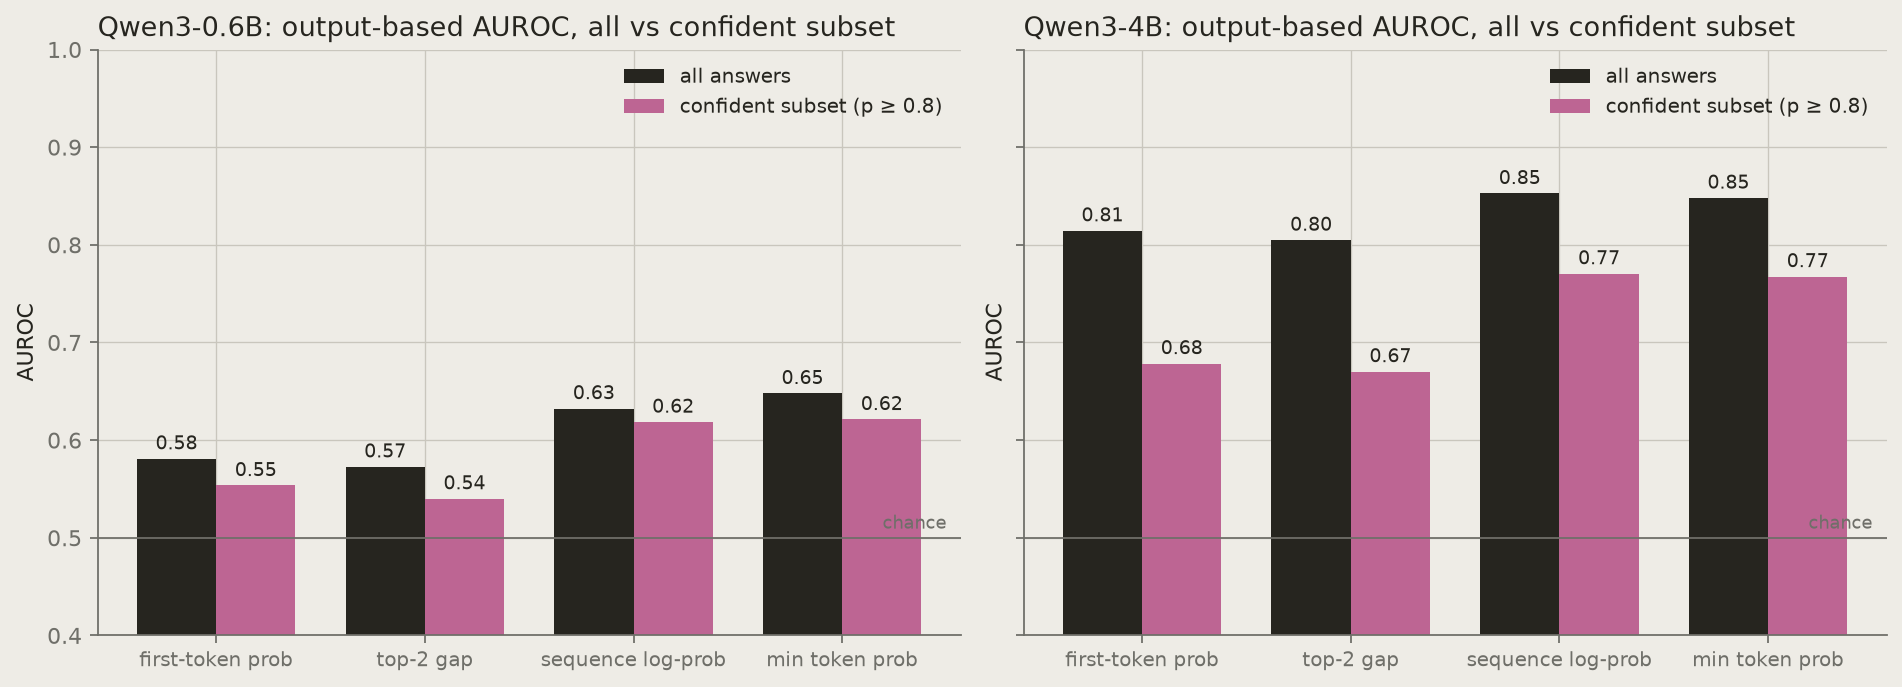
\includegraphics[width=0.98\textwidth]{04_output_auroc_all_vs_confident}
  \caption{AUROC of four output-side scores, on all answers (dark) and on the confident subset (pink). Every score drops when restricted to confident answers; first-token probability is at chance (0.55) on 0.6B. Notebook Figure 4.}
\end{figure}

Both models are overconfident everywhere (expected calibration error 0.47 and 0.33). Sequence log-probability is the strongest output score at 4B (0.85 overall), a fact that matters later.

\subsection{Semantic entropy recovers half of the confident errors, and no more}\label{sec:se}

\begin{figure}[H]\centering
  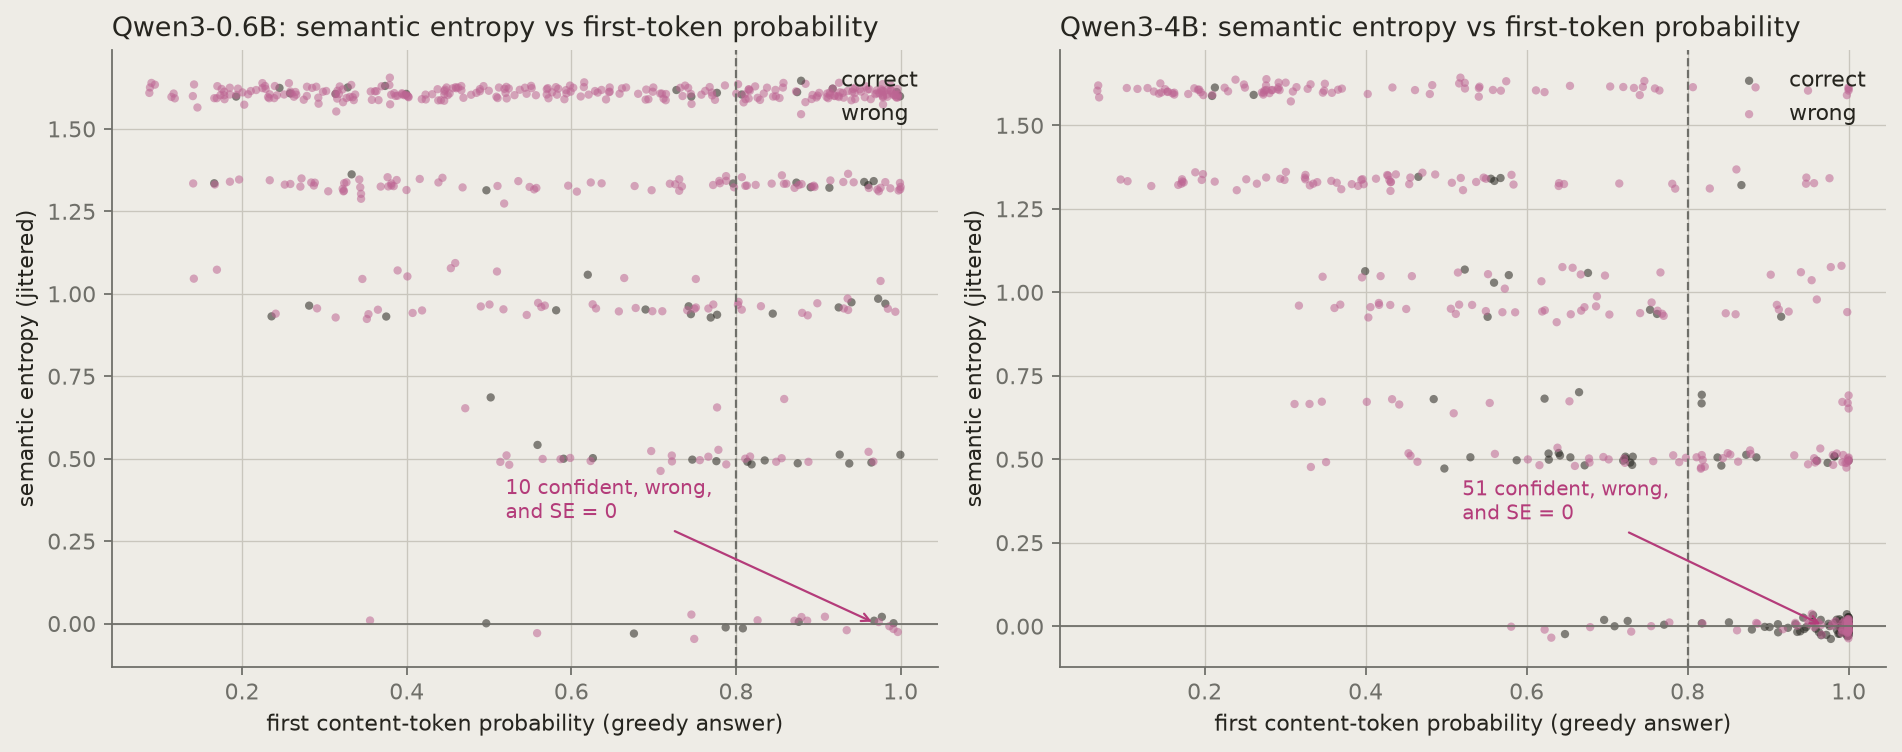
\includegraphics[width=0.98\textwidth]{06_se_vs_tokenprob_scatter}
  \caption{Semantic entropy against first-token probability, coloured by correctness. The signals agree on the easy region (low probability, high entropy). The bottom-right corner, high probability and zero entropy, is where both go quiet and still holds a pink population: 51 of 110 confident errors at 4B. Notebook Figure 6.}
\end{figure}

This refuted a prediction. We expected SE to be near-blind on confident answers; instead it scores 0.73 there at 4B against 0.62 for token probability, because confident errors are unstable under sampling more often than confident successes. What SE cannot see is the stable half. That stable, confident, wrong set is the hard set used below.

\begin{figure}[H]\centering
  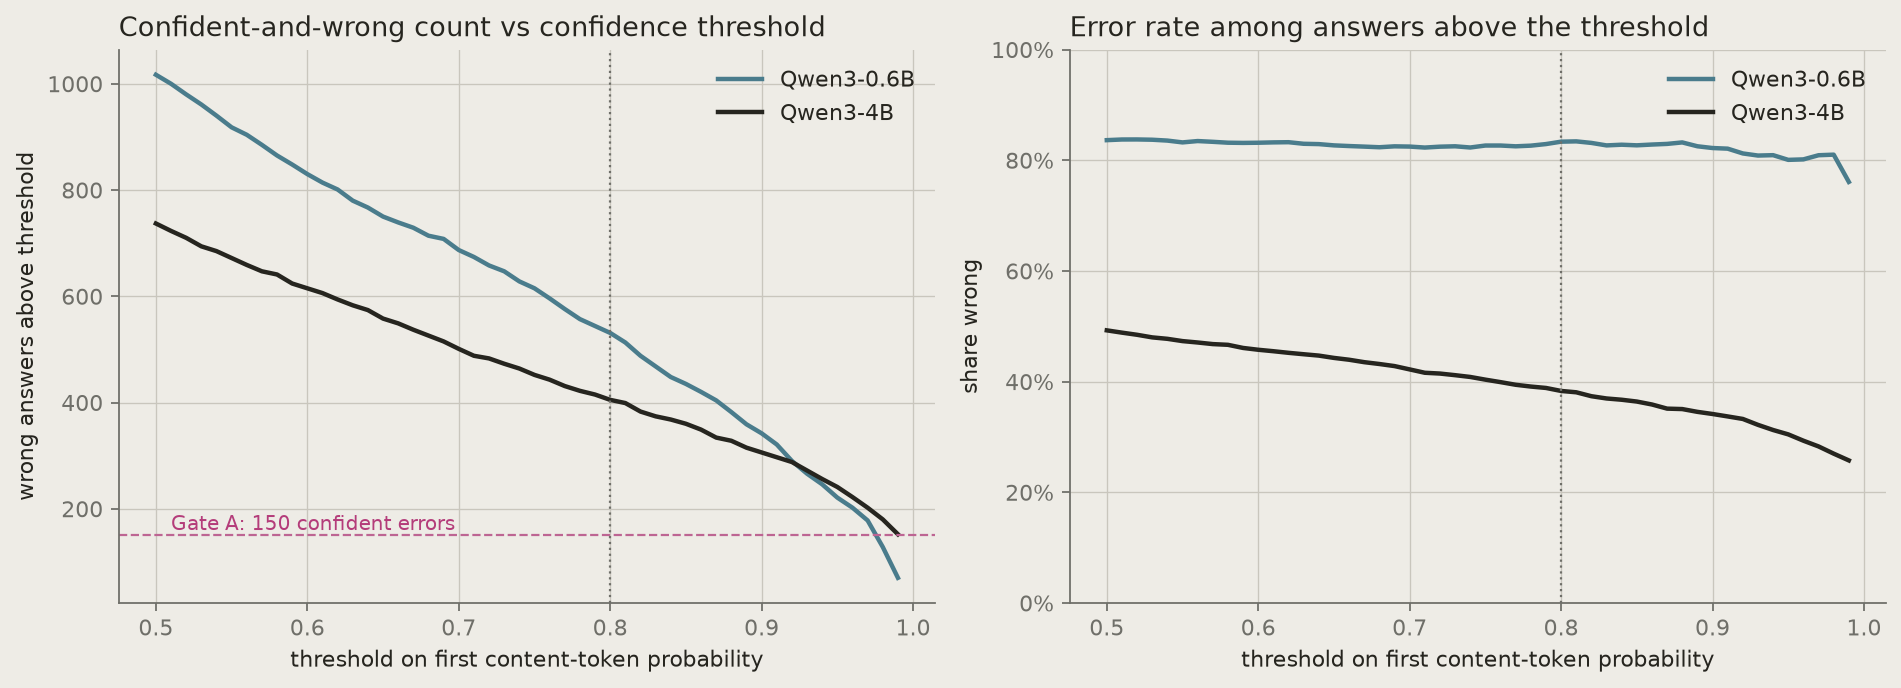
\includegraphics[width=0.98\textwidth]{11_threshold_sweep}
  \caption{The confident-error count and the error rate among confident answers as the threshold is raised from 0.5 to 0.99. At 0.6B the error rate does not move; raising the bar does not buy out of the problem. Notebook Figure 11.}
  \label{fig:sweep}
\end{figure}

\subsection{The internal signal survives where every output signal is exhausted (H1)}

\begin{figure}[H]\centering
  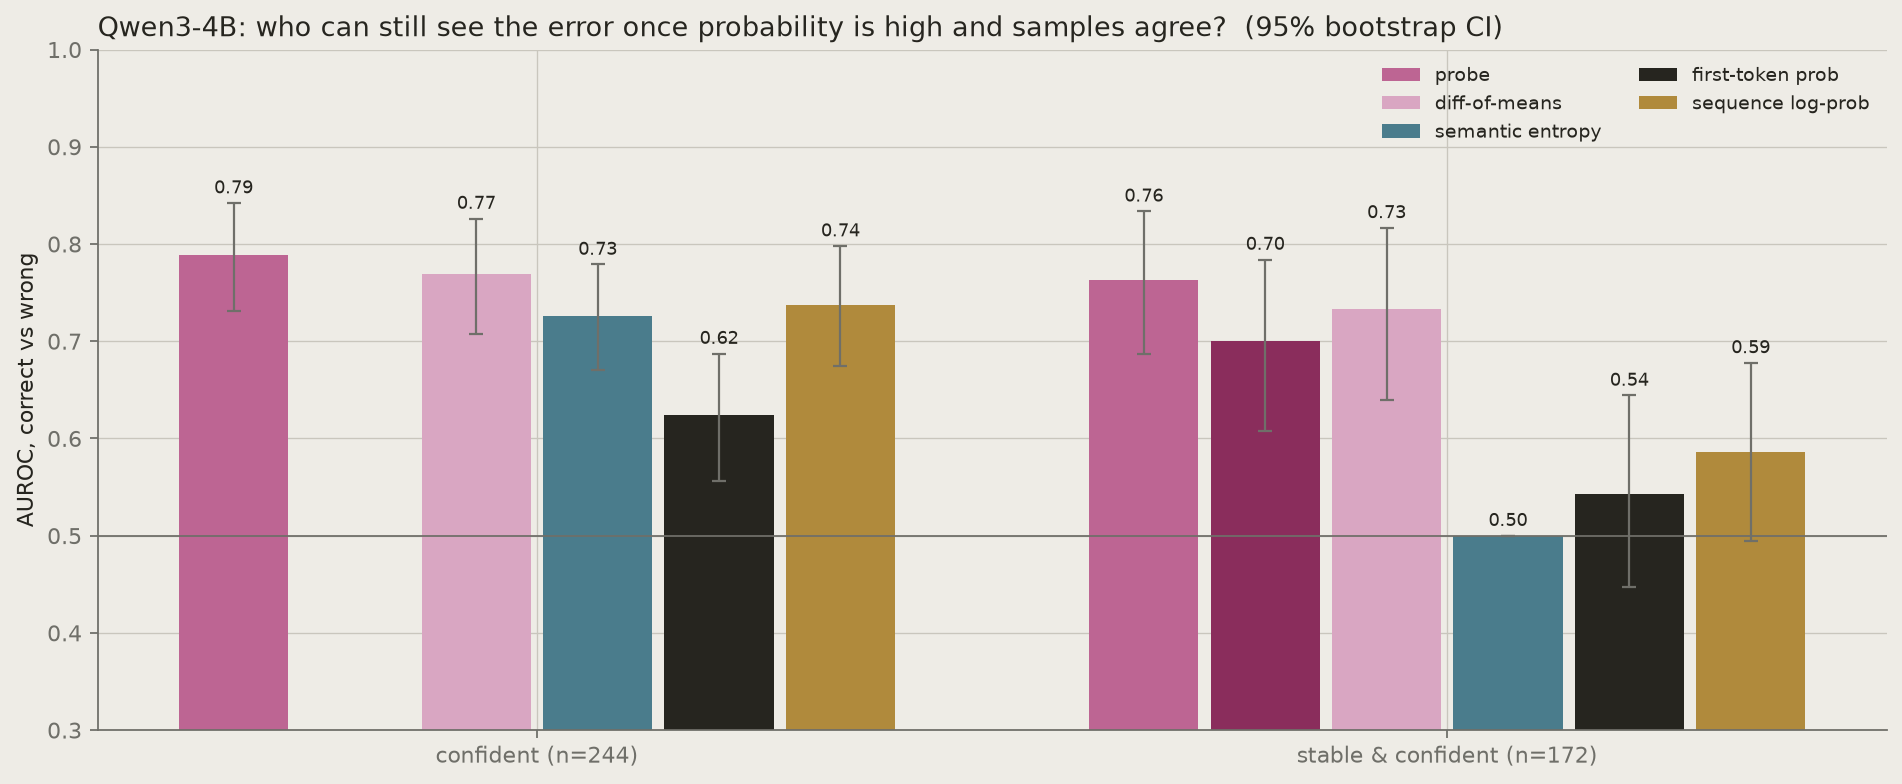
\includegraphics[width=0.98\textwidth]{18_hard_set_auroc}
  \caption{Qwen3-4B. Left group: the confident subset of the 500 sampled questions. Right group: the hard set, confident and SE $=0$. On the hard set the probe holds at 0.76 (CI 0.69--0.84), a probe trained \emph{only} inside the hard set at 0.70, and every output-side score at 0.50--0.59. Notebook Figure 18.}
\end{figure}

H1 passes as pre-registered on both models: the probe's lower bound clears the token-probability baseline on the confident subset (0.6B: 0.74 vs 0.55; 4B: 0.74 vs 0.68). The honest qualification is that sequence log-probability, which we did not pre-register, ties the probe on the confident subset at 4B (0.77). The hard set removes that ambiguity: there, nothing the model outputs ranks right above wrong, and the residual stream still does.

\subsection{Directions: distinct at 0.6B, shared at 4B (first look at H2)}\label{sec:directions}

\begin{figure}[H]\centering
  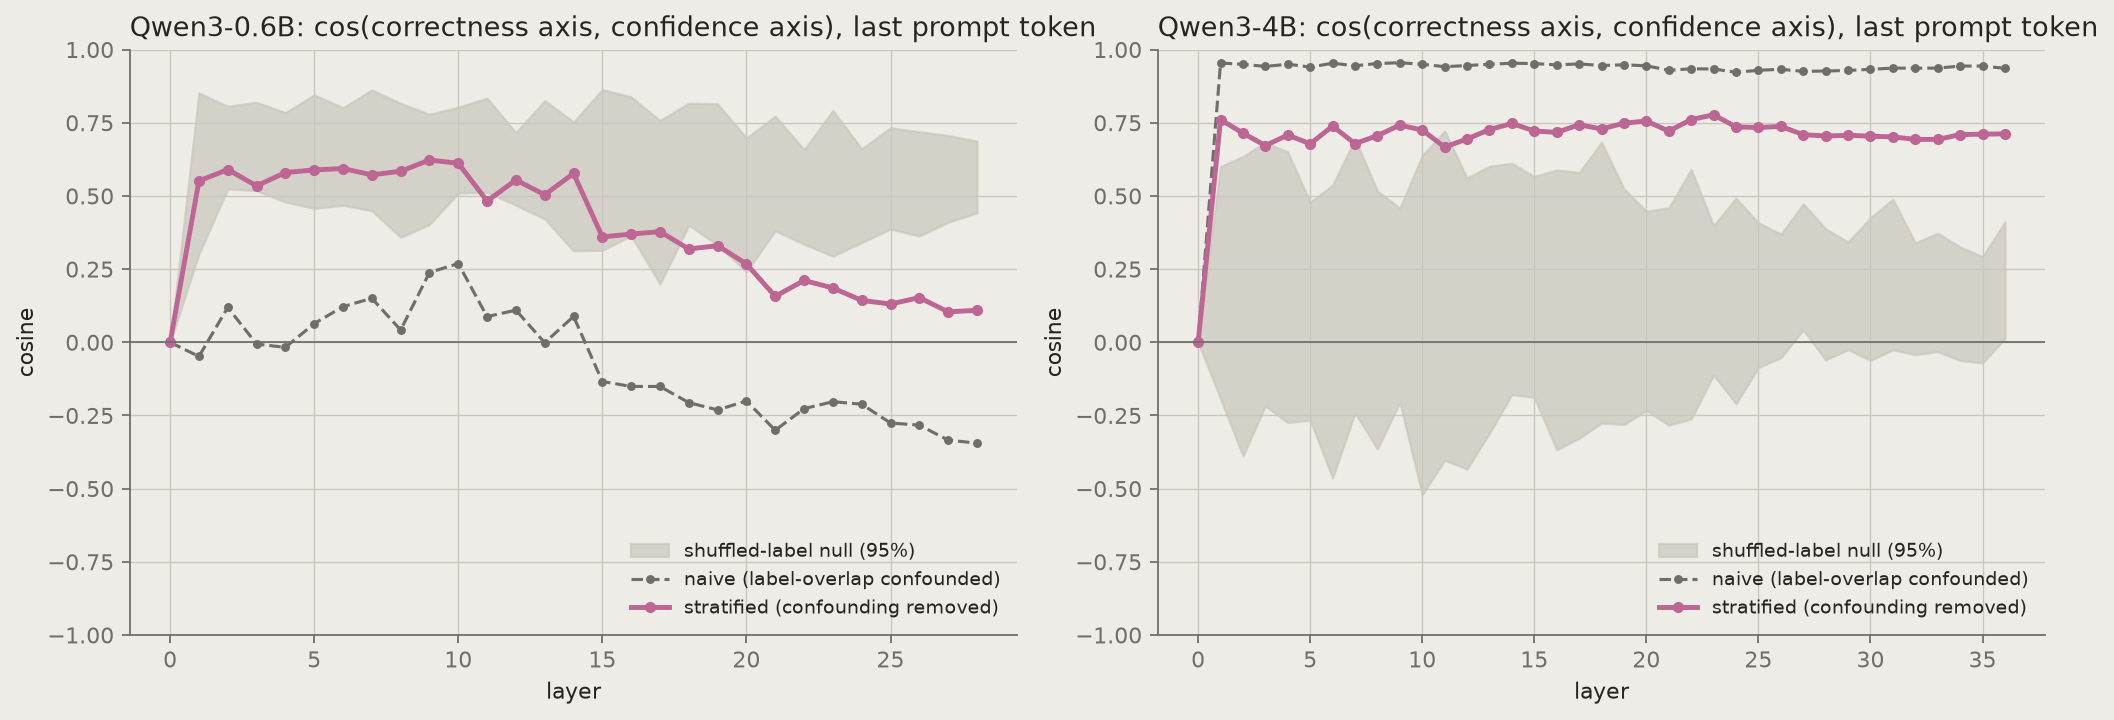
\includegraphics[width=0.98\textwidth]{20_axis_cosine_stratified}
  \caption{Cosine between the correctness axis (estimated within confident answers) and the confidence axis (estimated within correct answers), by layer. Grey dashed: the naive version, confounded by label overlap. Grey band: the same statistic with correctness labels shuffled. Notebook Figure 20.}
\end{figure}

\begin{figure}[H]\centering
  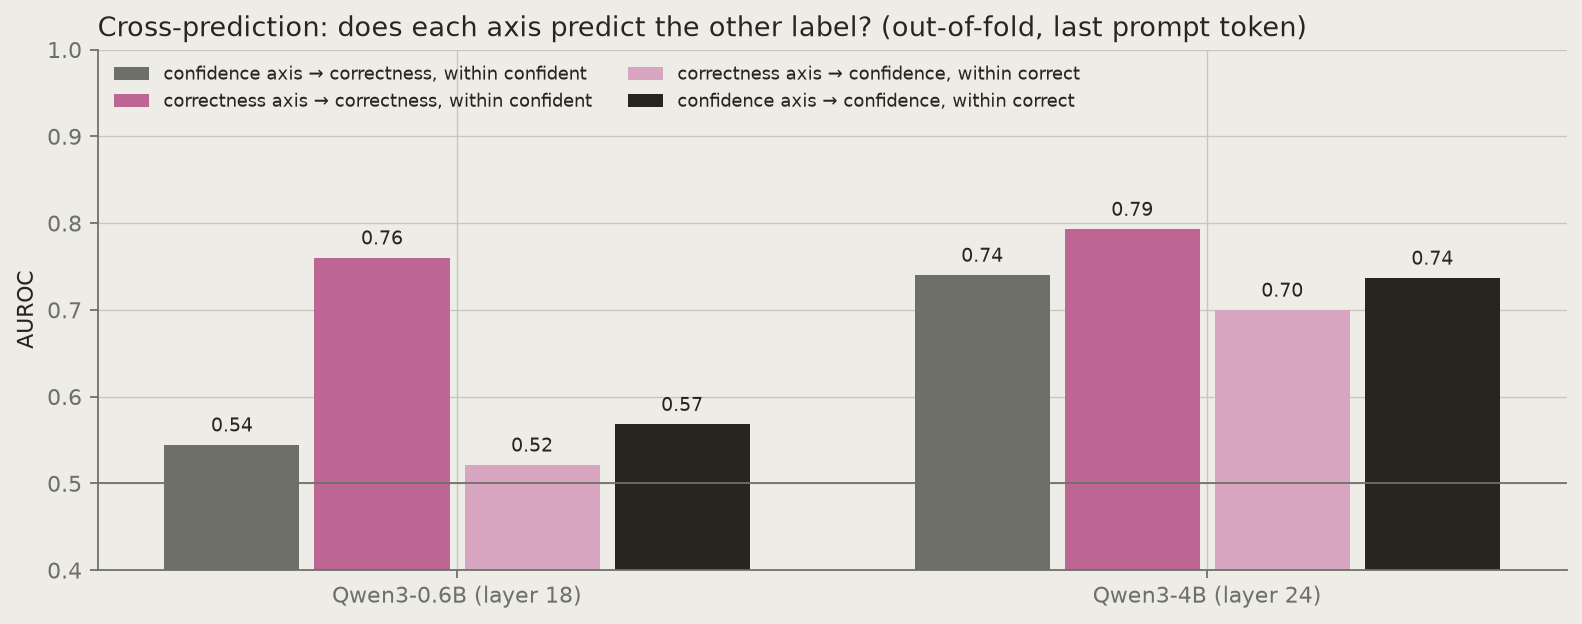
\includegraphics[width=0.85\textwidth]{21_axis_cross_prediction}
  \caption{Out-of-fold cross-prediction at the best layer. Pink: the correctness axis predicting correctness within confident answers. Grey: the confidence axis attempting the same. Notebook Figure 21.}
\end{figure}

Two findings. First, methodological: \textbf{the shuffled-label null for a residual-stream cosine is not centred on zero.} Mean-difference vectors live mostly in a few dominant directions, so two unrelated axes have cosine 0.3--0.7 by accident. Any CSO-style cosine criterion applied to hallucination needs a null of this kind, or whitening, before a high cosine means anything. Second, the models disagree. At 0.6B the correctness direction sits \emph{below} the null in later layers and the confidence axis barely predicts correctness (0.54 vs 0.76): wrongness has its own direction. At 4B the two axes are largely one feature (0.74 vs 0.79): the internal signal there is mostly an internal confidence the model carries but does not express in its output. Both are monitors the output cannot provide; only the first is the ``off-axis'' geometry CSO-LLM describes.

\section{What this tells us}

\begin{itemize}
  \item \textbf{About the literature.} Each paper's headline replicates qualitatively in a 4B model on a laptop: SE above token scores, a 20--27\% confident-wrong population, probes above output scores on confident answers with a mid-stack best layer. Two things the literature understates: output probability is a poor certainty proxy in small models, and residual-stream cosines carry a non-zero null.
  \item \textbf{About the hypothesis.} H1 holds and is sharpest on the hard set. H2 is model-dependent, which reframes it: the question for November is not ``is there a wrongness direction'' but ``under what conditions is it separable from confidence,'' tested per pair with the CHOKE protocol.
  \item \textbf{About the methodology.} Three corrections for the next phase. Define the population by sampling stability, not probability alone. Report sequence log-probability as the baseline, not first-token probability. Audit about 200 labels with an LLM judge before any number is quoted as final.
\end{itemize}

\section{Next steps to November 6}
\begin{enumerate}
  \item LLM-judge audit of 200 labels, stratified by quadrant, to bound the lexical-label effect \citep{janiak2025illusion}.
  \item CHOKE-style paired prompts on Qwen3-4B: the same question in two phrasings that flip the answer; per-pair displacement cosine against the confidence axis, with a shuffled null. This is the direct test of H2 in CSO-LLM's own terms.
  \item Transfer: probe trained on TriviaQA, tested on Natural Questions, to see whether the hard-set signal is task-general or task-specific.
\end{enumerate}

\bibliographystyle{plainnat}
{\small\bibliography{refs}}
\end{document}
